%% abtex2-modelo-trabalho-academico.tex, v-1.7.1 laurocesar
%% Copyright 2012-2013 by abnTeX2 group at http://abntex2.googlecode.com/ 
%%
%% This work may be distributed and/or modified under the
%% conditions of the LaTeX Project Public License, either version 1.3
%% of this license or (at your option) any later version.
%% The latest version of this license is in
%%   http://www.latex-project.org/lppl.txt
%% and version 1.3 or later is part of all distributions of LaTeX
%% version 2005/12/01 or later.
%%
%% This work has the LPPL maintenance status `maintained'.
%% 
%% The Current Maintainer of this work is the abnTeX2 team, led
%% by Lauro César Araujo. Further information are available on 
%% http://abntex2.googlecode.com/
%%
%% This work consists of the files abntex2-modelo-trabalho-academico.tex,
%% abntex2-modelo-include-comandos and abntex2-modelo-references.bib
%%

% ------------------------------------------------------------------------
% ------------------------------------------------------------------------
% abnTeX2: Modelo de Trabalho Academico (tese de doutorado, dissertacao de
% mestrado e trabalhos monograficos em geral) em conformidade com 
% ABNT NBR 14724:2011: Informacao e documentacao - Trabalhos academicos -
% Apresentacao
% ------------------------------------------------------------------------
% ------------------------------------------------------------------------

\documentclass[
	% -- opções da classe memoir --
	12pt,				% tamanho da fonte
	openright,			% capítulos começam em pág ímpar (insere página vazia caso preciso)
	twoside,			% para impressão em verso e anverso. Oposto a oneside
	a4paper,			% tamanho do papel. 
	% -- opções da classe abntex2 --
	%chapter=TITLE,		% títulos de capítulos convertidos em letras maiúsculas
	%section=TITLE,		% títulos de seções convertidos em letras maiúsculas
	%subsection=TITLE,	% títulos de subseções convertidos em letras maiúsculas
	%subsubsection=TITLE,% títulos de subsubseções convertidos em letras maiúsculas
	% -- opções do pacote babel --
	english,			% idioma adicional para hifenização
	brazil,				% o último idioma é o principal do documento
	]{abntex2}


% ---
% PACOTES
% ---

% ---
% Pacotes fundamentais 
% ---
\usepackage{cmap}				% Mapear caracteres especiais no PDF
\usepackage[T1]{fontenc}		% Selecao de codigos de fonte.
\usepackage[utf8]{inputenc}		% Codificacao do documento (conversão automática dos acentos)
\usepackage{lastpage}			% Usado pela Ficha catalográfica
\usepackage{indentfirst}		% Indenta o primeiro parágrafo de cada seção.
\usepackage{color}				% Controle das cores
\usepackage{graphicx}			% Inclusão de gráficos
\usepackage{xspace}
\usepackage{fourier} 
\usepackage{array}
\usepackage{makecell}
\usepackage{graphics}
% ---

% Pacotes extras
\usepackage[table,xcdraw]{xcolor}   % Inclusão de cores em tabelas
\usepackage{todonotes}
\usepackage{multirow}
\usepackage{pdfpages}
\usepackage{pgfgantt}
\usepackage{changepage}

% Abreviações
\newcommand{\Fw}{\textit{Framework}\xspace}
\newcommand{\fw}{\textit{framework}\xspace}
\newcommand{\Fws}{\textit{Frameworks}\xspace}
\newcommand{\fws}{\textit{frameworks}\xspace}

\newcommand{\pskel}{{\small \textsf{PSkel}}\xspace}
\newcommand{\mppa}{{\small \textsf{MPPA-256}}\xspace}
\newcommand{\charm}{{\small \texttt{Charm++}}\xspace}

% ---
% Pacotes adicionais, usados apenas no âmbito do Modelo Canônico do abnteX2
% ---
\usepackage{lipsum}				% para geração de dummy text
% ---

% ---
% Pacotes de citações
% ---
%\usepackage[brazilian,hyperpageref]{backref}	 % Paginas com as citações na bibl
\usepackage[alf]{abntex2cite}	                 % Citações padrão ABNT

% --- 
% CONFIGURAÇÕES DE PACOTES
% --- 

% ---
% Configurações do pacote backref
% Usado sem a opção hyperpageref de backref
%\renewcommand{\backrefpagesname}{Citado na(s) página(s):~}
% Texto padrão antes do número das páginas
%\renewcommand{\backref}{}
% Define os textos da citação
%\renewcommand*{\backrefalt}[4]{
%	\ifcase #1 %
%		Nenhuma citação no texto.%
%	\or
%		Citado na página #2.%
%	\else
%		Citado #1 vezes nas páginas #2.%
%	\fi}%
% ---

% ---
% Informações de dados para CAPA e FOLHA DE ROSTO
% ---
% nomes

\titulo{Abstração da Topologia de Rede para Aplicações Distribuídas}
\autor{Thales Alexandre Zirbel Hubner}
\local{Florianópolis}
\data{2018}
\orientador{Vinicius Marino Calvo Torres de Freitas}
\coorientador{Márcio Bastos Castro}
\instituicao{%
  Universidade Federal de Santa Catarina
  \par
  Departamento de Informática e Estatística
  \par
  Ciência da Computação}
\tipotrabalho{Trabalho de Conclusão de Curso de Graduação}
% O preambulo deve conter o tipo do trabalho, o objetivo, 
% o nome da instituição e a área de concentração 
\preambulo{Monografia submetida ao Programa
de Graduação em Ciência da Computação
para a obtenção do Grau de Bacharel.}
% ---


% ---
% Configurações de aparência do PDF final

% alterando o aspecto da cor azul
\definecolor{blue}{RGB}{41,5,195}

% informações do PDF
\makeatletter
\hypersetup{
     	%pagebackref=true,
		pdftitle={\@title}, 
		pdfauthor={\@author},
    	pdfsubject={\imprimirpreambulo},
	    pdfcreator={LaTeX with abnTeX2},
		pdfkeywords={abnt}{latex}{abntex}{abntex2}{trabalho acadêmico}, 
		hidelinks,
		colorlinks=false,       	% false: boxed links; true: colored links
    	linkcolor=blue,          	% color of internal links
    	citecolor=blue,        		% color of links to bibliography
    	filecolor=magenta,      	% color of file links
		urlcolor=blue,
		bookmarksdepth=4
}
\makeatother
% --- 

% --- 
% Espaçamentos entre linhas e parágrafos 
% --- 

% O tamanho do parágrafo é dado por:
\setlength{\parindent}{1.3cm}

% Controle do espaçamento entre um parágrafo e outro:
\setlength{\parskip}{0.2cm}  % tente também \onelineskip

% ---
% compila o indice
% ---
\makeindex
% ---

% ----
% Início do documento
% ----
\usepackage{times} 			% Usa a fonte Times
\begin{document}

% Retira espaço extra obsoleto entre as frases.
\frenchspacing 

% ----------------------------------------------------------
% ELEMENTOS PRÉ-TEXTUAIS
% ----------------------------------------------------------
% \pretextual

% ---
% Capa
% ---
\imprimircapa
% ---

% ---
% Folha de rosto
% (o * indica que haverá a ficha bibliográfica)
% ---
\imprimirfolhaderosto*
% ---

% ---
% Inserir folha de aprovação
% ---

% Isto é um exemplo de Folha de aprovação, elemento obrigatório da NBR
% 14724/2011 (seção 4.2.1.3). Você pode utilizar este modelo até a aprovação
% do trabalho. Após isso, substitua todo o conteúdo deste arquivo por uma
% imagem da página assinada pela banca com o comando abaixo:
%
% \includepdf{folhadeaprovacao_final.pdf}
%
\begin{folhadeaprovacao}
	%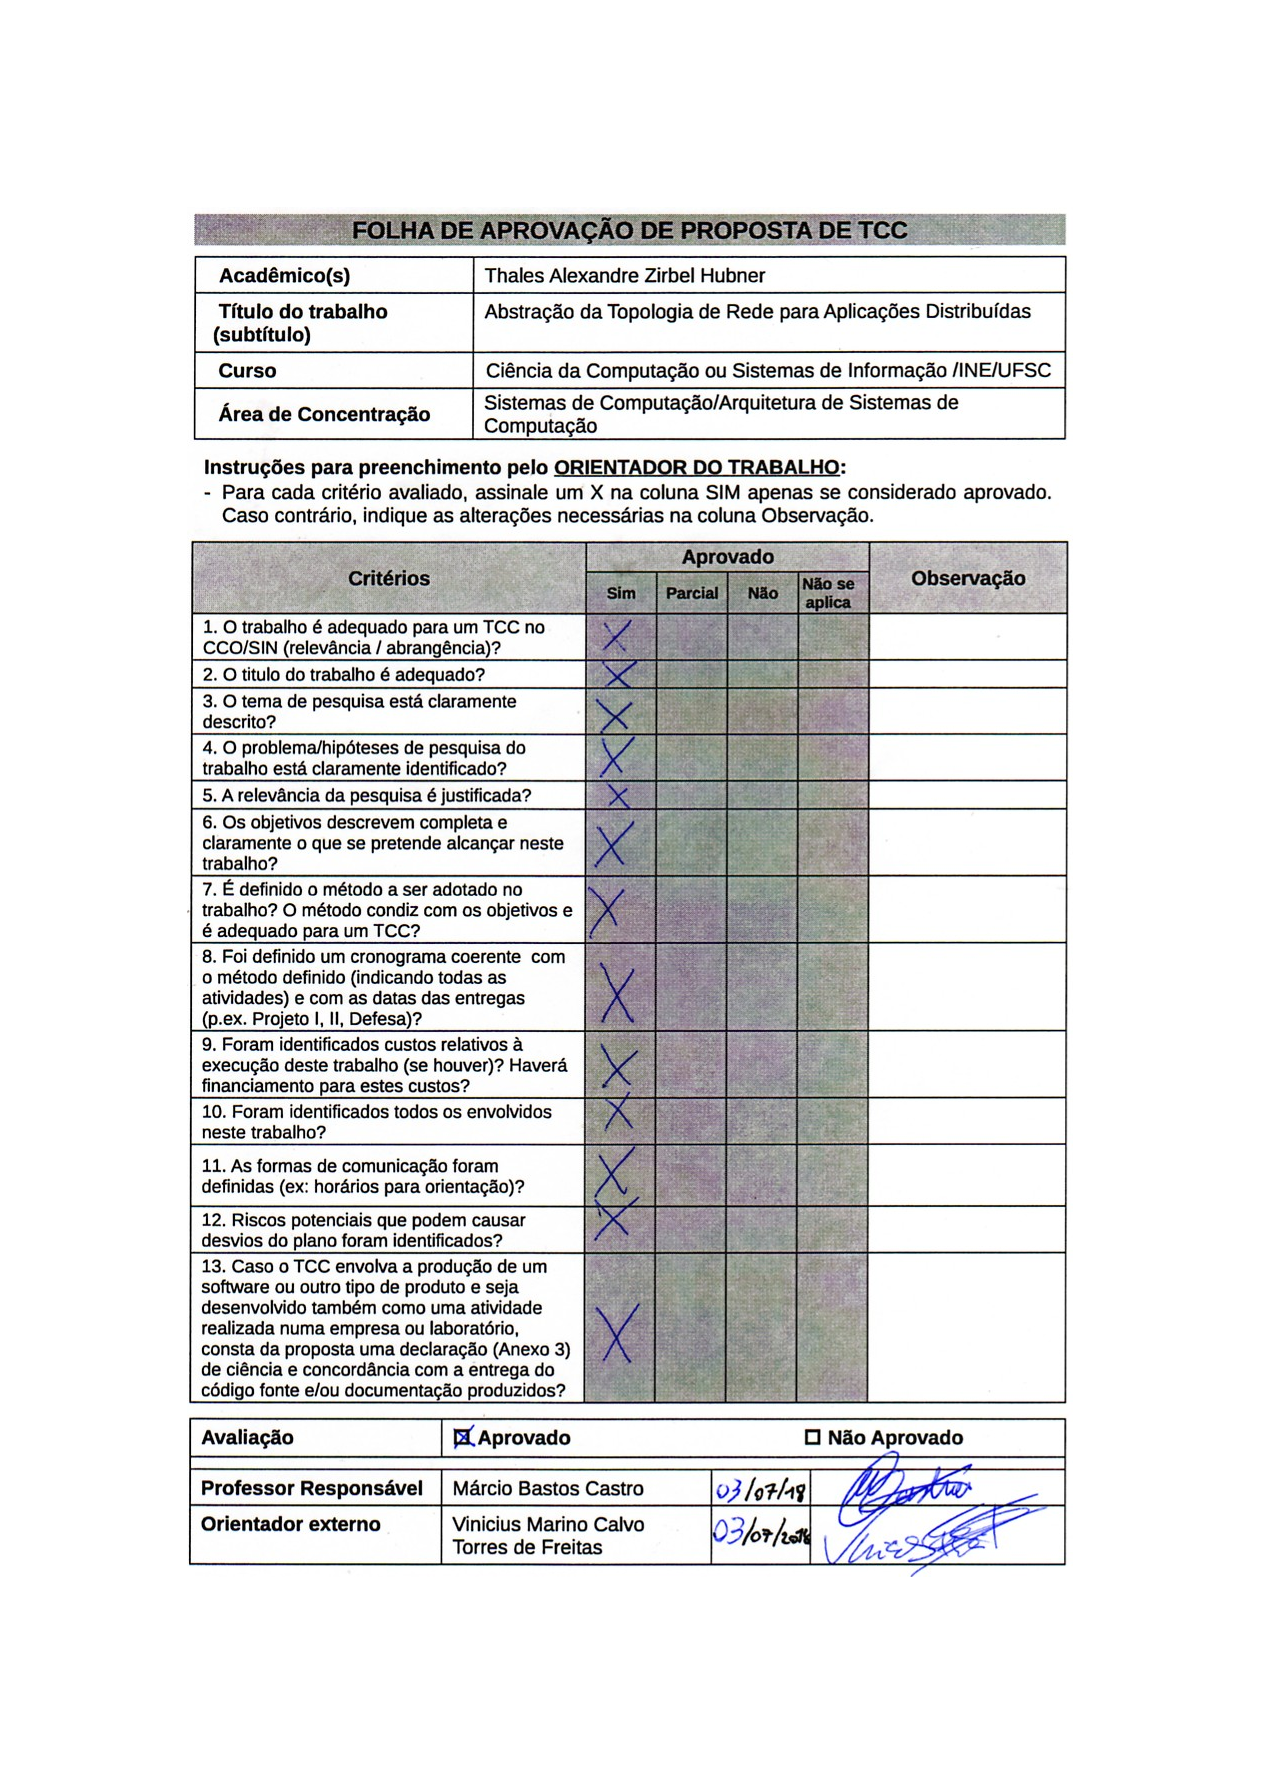
\includepdf{folha_aprovacao_assinada}  
\end{folhadeaprovacao}
% ---

% ---
% RESUMOS
% ---

% resumo em português
\begin{resumo}

A repartição de trabalho em ambientes distribuídos é um problema a ser tratado, pois aplicações como simulações sísmicas, dinâmica molecular e previsão de tempo possuem comportamento dinâmico, o que gera desbalanceamento de cargas de trabalho no sistema. Uma das maneiras de resolver esse problema é a utilização de balanceadores de carga dinâmicos, cuja função é reduzir o tempo de execução da aplicação através de uma distribuição de tarefas mais homogênea. A execução destes balanceadores gera um sobrecusto relacionado à comunicação para o balanceamento e à migração de tarefas. Poucos balanceadores consideram a topologia do sistema de maneira dinâmica, devido à dificuldade do balanceador de acessar as informações completas sobre a rede e de levá-las em consideração para o remapeamento de tarefas.

Este trabalho visa a implementação de uma abstração da topologia de rede, facilitando o acesso à métricas mais complexas da rede e a utilização destas em aplicações distribuídas. Por cima dessa abstração, será implementado uma estratégia de balanceamento de carga que utilizará a informação de custos heterogêneos de comunicação na rede, reduzindo o sobrecusto de comunicação através do uso de partes mais velozes da rede. Este balanceador será comparado com outros balanceadores de carga que não utilizam desta informação, verificando sua efetividade em cenários heterogêneos e seu sobrecusto em cenários homogêneos.


%  Segundo a \citeonline[3.1-3.2]{NBR6028:2003}, o resumo deve ressaltar o
%  objetivo, o método, os resultados e as conclusões do documento. A ordem e a extensão
%  destes itens dependem do tipo de resumo (informativo ou indicativo) e do
%  tratamento que cada item recebe no documento original. O resumo deve ser
%  precedido da referência do documento, com exceção do resumo inserido no
%  próprio documento. (\ldots) As palavras-chave devem figurar logo abaixo do
%  resumo, antecedidas da expressão Palavras-chave:, separadas entre si por
%  ponto e finalizadas também por ponto.\citeonline{Emma}.\citeonline{Nielsen}.
%  \citeonline{Goodfellow-et-al-2016}

 \vspace{\onelineskip}
    
 \noindent
 \textbf{Palavras-chaves}: topologia de rede. balanceamento de carga. aplicações distribuidas.
 
\end{resumo}

% resumo em inglês
% \begin{resumo}[Abstract]
%  \begin{otherlanguage*}{english}
%    This is the english abstract.

%    \vspace{\onelineskip}
 
%    \noindent 
%    \textbf{Key-words}: latex. abntex. text editoration.
%  \end{otherlanguage*}
% \end{resumo}

% ---
% inserir lista de ilustrações
% ---
%\pdfbookmark[0]{\listfigurename}{lof}
%\listoffigures*
%\cleardoublepage
% ---

% ---
% inserir lista de tabelas
% ---
%\pdfbookmark[0]{\listtablename}{lot}
%\listoftables*
%\cleardoublepage
% ---

% ---
% inserir lista de abreviaturas e siglas
% ---
\begin{siglas}
  \item[PE] \textit{Processing Element}, unidade de processamento
  \item[LB] \textit{Load Balancer}, balanceador de carga
\end{siglas}
% ---

% ---
% inserir lista de símbolos
% ---
%\begin{simbolos}
%  \item[$ \Gamma $] Letra grega Gama
%  \item[$ \Lambda $] Lambda
%  \item[$ \zeta $] Letra grega minúscula zeta
%  \item[$ \in $] Pertence
%\end{simbolos}
% ---

% ---
% inserir o sumario
% ---
\pdfbookmark[0]{\contentsname}{toc}
\tableofcontents*
\cleardoublepage
% ---



% ----------------------------------------------------------
% ELEMENTOS TEXTUAIS
% ----------------------------------------------------------
\textual


% ----------------------------------------------------------
% Introdução
% ----------------------------------------------------------
\chapter{Projeto}

Este capítulo apresenta o tema de pesquisa do Trabalho de Conclusão de Curso, o escopo no qual o problema em questão será tratado e a justificativa do projeto. Na Seção \ref{sec:introducao} é apresentado o contexto e a motivação para a realização do trabalho. Na Seção \ref{sec:objetivos} são introduzidos os objetivos gerais e específicos, as restrições e premissas existentes, a lista de marcos e os critérios de aceite do projeto. Na Seção \ref{sec:metodologia}, são abordados os métodos de pesquisa envolvidos para alcançar a solução proposta.


\section{Introdução}
\label{sec:introducao}

Aplicações no âmbito científico e industrial incluem cada vez mais detalhes, demandam precisão ainda maior e/ou possuem uma complexidade muito elevada, criando uma demanda cada vez maior por velocidade e poder de processamento~\cite{pilla-thesis}. Uma das maneiras utilizadas para suprir esta demanda é com computação paralela, que alcança a solução destes problemas através da repartição de trabalho entre unidades de processamento (\textit{Processing Elements} ou PE's) e a execução destas parcelas simultâneamente. Este método permite que um aumento no número de PE’s leve a uma redução no tempo da aplicação. Contudo a melhoria no tempo é limitada pela parcela não paralelizável do programa e pelos recursos do sistema~\cite{amdahl}. 

Supercomputadores que utilizam da computação paralela foram criados para alcançar processamento massivo e por décadas estas máquinas cresceram. Elas alcançaram um ponto onde se percebeu que velocidade e poder de processamento não eram as métricas adequadas para desempenho destas máquinas. Estes computadores consomem uma quantidade tremenda de energia e dissipam muito desta energia, se tornando grandes geradores de calor~\cite{green500}. A geração de calor excessiva é um problema em sistema pois temperaturas altas aumentam sua chance de falha e tempo fora de operação. Como contramedida é necessário a implantação de um sistema eficiente de redução de temperatura, que traz outro grande sobrecusto de energia. Com estes problemas em mente a métrica pensada para estas máquinas é a eficiência de processamento, que leva em conta a energia gasta no sistema, a velocidade e o poder de processamento~\cite{efficient-metric}.

Uma das opções para obter eficiência de processamento é o uso de um número maior de núcleos menos potentes~\cite{snir-encyclopedia}. A organização de um número tão grande de PE’s acaba levando a um sistema com memória distribuída, que operam com o uso de diversas máquinas e utilizam alguma rede para a interligação e comunicação. A escolha destes sistemas é devida ao seu custo baixo e a sua grande escalabilidade através do aumento no número de máquinas. O contraponto destas vantagens é o desenvolvimento destas aplicações, que se torna mais complexo pois têm de levar em consideração fatores impactantes como sincronização, dependência e distribuição de dados, balanceamento de carga e custos de comunicação~\cite{pilla-thesis}.

A repartição de trabalho em ambientes distribuídos é um problema a ser tratado, pois aplicações como simulações sísmicas~\cite{dupros}~\cite{tesser}, dinâmica molecular~\cite{bathele-kale} ou previsão de tempo~\cite{rodrigues} possuem comportamento dinâmico, ou seja suas cargas mudam ao longo da execução da aplicação, levando um mapeamento homogêneo de tarefas a um estado desbalanceado do sistema, resultando em uma subcarga de alguns PE’s. Esta subcarga resulta no sub-uso de processadores e na possibilidade de alguns PE's não terem trabalho para executar, reduzindo o desempenho da aplicação. Para consertar tais desvios pode-se usar um balanceador de carga (\textit{Load Balancer} ou LB) dinâmico, cujo trabalho é remapear as tarefas entre os PE’s, buscando um estado mais balanceado do sistema. Este rearranjo garante a utilização dos PE's de maneira mais homogênea e leva a uma redução do tempo da aplicação.

Os PE’s em sistemas distribuídos se comunicam usando diversas topologias de rede, como malhas, tori ou \textit{fat-trees}. Os PE's utilizam de \textit{links} de conexão da rede para efetuar sua comunicação. O compartilhamento destes pode resultar num congestionamento da rede devido ao sobreuso de alguns \textit{links}~\cite{bathele-encyclopedia}. Outro fator é a possibilidade da rede não ter ligações com custos iguais comunicação~\cite{dragonfly}, tendo variações de latência e velocidade em partes distintas da rede. O impacto disto é que os caminhos menos custosos entre PE's da rede nem sempre são os menores em questão de \textit{links} percorridos. 

Os caminhos utilizados dentro de uma rede têm impacto no tempo de execução de um programa, pois caminhos mais lentos afetam o sobrecusto de comunicação. É possível que um LB leve em conta os custos de comunicação entre os PE's e os custos de movimentação destas tarefas dentro da rede. Tal abordagem pode levar a uma redução do custo de comunicação, evitando a troca de informação e tarefas através de partes lentas da rede.

\section{Objetivos}
\label{sec:objetivos}

Os objetivos deste trabalho são de desenvolver uma abstração da topologia de rede, facilitando seu uso para outras aplicações e propor uma estratégia de balanceamento de carga ciente desta abstração. Para este fim, seguem os objetivos específicos:

\begin{enumerate}
\item Desenvolver um método de abstração dinâmica da topologia de rede para a plataforma Charm++~\cite{website:CHARM};
\item  Desenvolver um LB que utilize esta base, visando a otimização para redes com custos de hops heterogêneos;
\item Testar e comparar este balanceador com outros LB's, dentro de sistemas com topologia de rede com custos de hop heterogêneo.
\end{enumerate}

\begin{flushleft}
\textbf{Premissas:}
\begin{itemize}
\item Um computador estará disponível para realização do trabalho; 
\item O orientador terá disponibilidade para reuniões periódicas;
\item Disponibilidade de energia e internet.
\item Acesso a uma máquina com uma topologia diferenciada para a realização dos testes.
\end{itemize}

\textbf{Marcos:}
\begin{itemize}
 
\item Entrega do resumo em TCC I: 4ª semana de Novembro/2018; 
\item Entrega da abstração da topologia: 4ª semana de Novembro/2018;
\item Entrega da implementação do balanceamento de carga: 4ª semana de Abril/2019;
\item Entrega da primeira versão da monografia em TCC II: 2ª semana de Maio/2019; 
\item Defesa da monografia: 2ª semana de Junho/2019;
\item Entrega da versão final da monografia em TCC II: 4ª semana de Junho/2019.
\end{itemize}

\textbf{Critérios de aceite:}
\begin{itemize}
\item Aprovação da banca avaliadora;
\item Aprovação do orientador;
\item Aprovação do coorientador;
\item Conformidade da monografia com as normas definidas pela instituição;
\item Prazos cumpridos.
\end{itemize}
\end{flushleft}

\section{Método de Pesquisa}
\label{sec:metodologia}

 
O ínicio do trabalho terá duas partes: uma de cunho teórico, onde será estudada a base e o estado da arte para o projeto, e outra mais prática, que envolve o aprendizado do \textit{framework} Charm++. A primeira parcela será constituída por um estudo sobre topologia de rede e balanceamento de carga em aplicações paralelas, criando uma base para o projeto. A segunda parte terá foco no entendimento da plataforma e suas nuances, visando facilitar a implementação da abstração.

A criação da abstração da topologia de rede utilizará a linguagem de programação C++ e será realizada dentro do \textit{framework} de programação paralela Charm++. A plataforma será utilizada pois têm uma base sólida para a criação, utilização e teste de balanceadores de carga e outras aplicações paralelas~\cite{pilla:CHARM}. Além disto Charm++ contém somente abstrações de topologia fixas, carecendo de uma abstração elaborada da topologia de rede, proposta neste trabalho.

Após a criação e teste da abstração da topologia de rede, será desenvolvido um LB que utiliza desta abstração para reduzir o custo de comunicação dentro de uma rede com custos de comunicação heterogêneos. O balanceador também será realizado em C++ na plataforma Charm++. Serão executados testes de funcionamento e avaliação de desempenho.

Na última etapa será realizado uma análise de desempenho do LB em comparação com outros LB's, verificando sua efetividade e seu sobrecusto como balanceador de carga. Para tal, serão realizados experimentos utilizando algum \textit{benchmark} que simule aplicações reais. O teste será realizado em um cenário onde a topologia tem custos de comunicação heterogêneos e outra com custos homogêneos. Também será realizado um teste para verificar o sobrecusto do LB em um cenário onde não há benefícios em balanceamento de carga.

% ----------------------------------------------------------
% PARTE - preparação da pesquisa
% ----------------------------------------------------------
% \part{Preparação da pesquisa}

% ----------------------------------------------------------
% Capitulo com exemplos de comandos inseridos de arquivo externo 
% ----------------------------------------------------------

\include{abntex2-modelo-include-comandos}

% ----------------------------------------------------------
% Parte de revisãod e literatura
% ----------------------------------------------------------
% \part{Revisão de Literatura}

% ---
% Capitulo de revisão de literatura
% ---
\def\coordenador{Renato Cislaghi}
\def\orientador{Vinicius Marino Calvo Torres de Freitas}
\def\coorientador{Márcio Bastos Castro}
\def\autor{Thales Alexandre Zirbel Hubner}

\chapter{Planejamento}

Este capítulo contém o planejamento do projeto onde cada parte do plano de gerenciamento se encontra em seções diferentes. A Seção \ref{sec:cronograma} apresenta as atividades planejadas e seu cronograma a ser seguido ao longo da realização deste trabalho. A Seção \ref{sec:rh} apresenta os recursos humanos envolvidos. A Seção \ref{sec:custos} indica os custos estimados para a execução do projeto. A Seção \ref{sec:comunicacao} dispõe o gerenciamento da comunicação entre as partes envolvidas. A Seção \ref{sec:riscos} apresenta os riscos identificados e suas respectivas estratégias.

% ---
\section{Cronograma}
\label{sec:cronograma}

As atividades previstas no projeto estão descritas abaixo:

\begin{itemize}
	\item \textbf{A1: Estudo da fundamentação teórica.} Nesta parte inicial será realizada a revisão de artigos e materiais relacionados a computação paralela, topologia de rede e balanceamento de carga.
	\item \textbf{A2: Familiarização com a plataforma charm++.} Processo de familiarização com a plataforma para programação paralela a ser utilizada.
	\item \textbf{A3: Revisão do estado da arte e prática.} Nesta etapa será tratada a revisão do estado da arte envolvido no contexto do trabalho, a fim de  fortalecer a base do conhecimento necessária para a realização do mesmo.
	\item \textbf{A4: Elaboração da proposta.} Nesta etapa será apresentada a proposta de solução do problema em questão, bem como suas estratégias de implementação.
	\item \textbf{A5: Escrita do relatório do TCC I.} Nesta etapa será realizada a escrita do relatório do TCC I. A entrega deste documento está prevista para a quarta semana do mês de novembro.
	\item \textbf{A6: Implementação da abstração da topologia de rede.} Nesta parcela será realizada a implementação da abstração proposta assim como a verificação do funcionamento desta.
	\item \textbf{A7: Teste da abstração da topologia de rede.} Nesta parcela será realizada a verificação do funcionamento da abstração.
	\item \textbf{A8: Desenvolvimento de um balanceador de carga.} Nesta etapa será efetuada o desenvolvimento de um balanceador de carga que utilize a abstração de rede criada.
	\item \textbf{A9: Testes e comparações de desempenho.} Nesta etapa será efetuado testes de desempenho do balanceador de carga a a comparação deste com outros balanceadores existentes.
	\item \textbf{A10: Escrita do rascunho do TCC II.} A escrita do rascunho do TCC II será realizada neste período. A entrega deste documento está prevista para a segunda semana do mês de maio.
	\item \textbf{A11: Preparação da defesa pública.} Nesta etapa será realizada a preparação da apresentação oral e visual do conteúdo deste trabalho para a defesa pública.
	\item \textbf{A12: Defesa pública.} Nesta etapa será realizada a defesa do projeto desenvolvido. Pretende-se realizar a defesa pública do trabalho na primeira semana do mês de junho.
	\item \textbf{A13: Correções e entrega da versão final do TCC.} Nesta etapa serão realizadas as correções e os ajustes da monografia e a entrega final do documento. A entrega da versão final está prevista para a quarta semana do mês de junho.
\end{itemize}

A Figura~\ref{fig:cronograma} apresenta o cronograma previsto para a realização das atividades descritas anteriormente. As atividades estão distribuídas ao longo do primeiro e segundo semestres de 2018 e o primeiro semestre de 2019.

% \begin{adjustwidth}{-2.5cm}{}
  \begin{figure}[h]
    \begin{center}
     \begin{ganttchart}[
       y unit title=0.4cm,
       y unit chart=0.6cm,
       hgrid,
       vgrid={{dotted, dotted, dotted, black}},
       title label font=\scriptsize,
       title/.append style={fill=gray!30},
       title height=1,
       bar/.append style={fill=gray!30,rounded corners=2pt},
       bar label font=\scriptsize,
       group label font=\scriptsize,
     ]{1}{30}
     	\gantttitle{\textbf{2018}}{18}
	 \gantttitle{\textbf{2019}}{12}\\
	 	\gantttitle{\textbf{Abr}}{2}
	 	\gantttitle{\textbf{Mai}}{2}
	 	\gantttitle{\textbf{Jun}}{2}
	 	\gantttitle{\textbf{Jul}}{2}
	 	\gantttitle{\textbf{Ago}}{2}
	 	\gantttitle{\textbf{Set}}{2}
	 	\gantttitle{\textbf{Out}}{2}
		\gantttitle{\textbf{Nov}}{2}						\gantttitle{\textbf{Dez}}{2}
     \gantttitle{\textbf{Jan}}{2}
	 \gantttitle{\textbf{Fev}}{2}
	 \gantttitle{\textbf{Mar}}{2}
	 \gantttitle{\textbf{Abr}}{2}
	 \gantttitle{\textbf{Mai}}{2}
	 \gantttitle{\textbf{Jun}}{2
}\\
     
     \ganttbar{A1}{1}{6} \\
     \ganttbar{A2}{2}{8} \\
     \ganttbar{A3}{5}{7} \\
     \ganttbar{A4}{5}{7} \\
     \ganttbar{A5}{9}{16} \\
     \ganttbar{A6}{9}{14} \\
     \ganttbar{A7}{14}{16} \\
     \ganttbar{A8}{16}{22} \\
     \ganttbar{A9}{22}{26} \\
     \ganttbar{A10}{24}{27} \\
     \ganttbar{A11}{26}{29} \\
     \ganttbar{A12}{29}{29} \\
     \ganttbar{A13}{29}{30}
     \end{ganttchart}
%  \end{adjustwidth}
     \caption{Cronograma de atividades.}\label{fig:cronograma}
  \end{center}
\end{figure}
% ---

% ---
\section{Recursos Humanos}
\label{sec:rh}
\begin{center}
\begin{tabular}{|c|c|}
\hline
    Papel & Nome \\ \hline
    Orientador & \orientador \\ \hline
    Coorientador & \coorientador \\ \hline
    Coordenador & \coordenador \\ \hline
    Membro da Banca I & \\ \hline
    Membro da Banca II & \\ \hline
    Autor & \autor \\ \hline
\end{tabular}
\end{center}
% ---
% ---
\section{Custos}
\label{sec:custos}

\begin{center}
\begin{tabular}{|c|c|c|c|c|c|}
\hline
\multicolumn{6}{|c|}{Estimativas para Recursos Humanos} \\ \hline
    Nome & Data Início & Data Fim & Hora/Mês & Valor/Hora & Custo Total \\ \hline
    Autor & 01/04/2018 & 01/06/2019 & 40 & R\$ 15,00 & R\$ 8400,00 \\ \hline
    Orientador & 01/04/2018 & 01/06/2019 & 4 & R\$ 20,00 & R\$ 1120,00 \\ \hline
    Coorientador & 01/04/2018 & 01/06/2019 & 4 & R\$ 71,00 & R\$ 3976,00 \\ \hline
    Coordenador & 01/04/2018 & 01/06/2019 & 1 & R\$ 102,00 & R\$ 1428,00 \\ \hline
    Membro da Banca I & 01/05/2019 & 01/06/2019 & 1 & R\$ 60,00 & R\$ 60,00 \\ \hline
    Membro da Banca II & 01/05/2019 & 01/06/2019 & 1 & R\$ 60,00 & R\$ 60,00 \\ \hline
\multicolumn{5}{|l|}{Subtotal estimativas para recursos humanos} & R\$ 15044,00 \\
\hline
\end{tabular}
\end{center}

\begin{center}
\resizebox{\textwidth}{!}{
    \begin{tabular}{|c|c|c|c|c|c|}
    \hline
    \multicolumn{6}{|c|}{Estimativas para Recursos Não Humanos} \\ \hline
        Descrição & Data Início & Data Fim & Quantidade & Valor Unitário & Custo Total \\
        \hline
        Computador para uso & 04/18 & 06/19 & 1 & R\$ 2500,00 & R\$ 2500,00 \\ \hline
        CDs para o código desenvolvido & 06/19 & 06/19 & 2 & R\$ 4,00 & R\$ 8,00 \\ \hline
        Impressão para o relatório & 12/18 & 12/18 & 3 & R\$ 20,00 & R\$ 60,00 \\ \hline
    \multicolumn{5}{|l|}{Subtotal estimativas para recursos não humanos} & R\$ 2568,00 \\
    \hline
    \end{tabular}
}
\end{center}
% ---

% ---
\section{Comunicação}
\label{sec:comunicacao}

\begin{center}
\begin{tabular}{|l|p{9cm}|}
\hline
    O que precisa ser comunicado & Reuniões periódicas com o Orientador e Coorientador\\ \hline
    Emissor & \autor \\ \hline
    Receptor & \orientador, \coorientador \\ \hline
    Comunicação & Reuniões periódicas com o Orientador para acompanhamento do projeto\\ \hline
    Forma de comunicação & Pessoalmente \\ \hline
    Frequência ou Quando & Quinzenalmente \\ \hline
\end{tabular}
\end{center}

\begin{center}
\begin{tabular}{|l|p{9cm}|}
\hline
    O que precisa ser comunicado & Entrega da Proposta \\ \hline
    Emissor & \autor \\ \hline
    Receptor & \coordenador \\ \hline
    Comunicação & Entrega da proposta completa do TCC \\ \hline
    Forma de comunicação & Sistema de TCC \\ \hline
    Frequência ou Quando & Única vez \\ \hline
\end{tabular}
\end{center}

\begin{center}
\begin{tabular}{|l|p{9cm}|}
\hline
    O que precisa ser comunicado & Entrega do Relatório em TCC I \\ \hline
    Emissor & \autor \\ \hline
    Receptor & \coordenador \\ \hline
    Comunicação & Entrega da primeira parte da monografia \\ \hline
    Forma de comunicação & Sistema de TCC \\ \hline
    Frequência ou Quando & Única vez \\ \hline
\end{tabular}
\end{center}

\begin{center}
\begin{tabular}{|l|p{9cm}|}
\hline
    O que precisa ser comunicado & Entrega da primeira versão da monografia completa em TCC II \\ \hline
    Emissor & \autor \\ \hline
    Receptor & \coordenador \\ \hline
    Comunicação & Entrega da primeira versão da monografia completa \\ \hline
    Forma de comunicação & Sistema de TCC \\ \hline
    Frequência ou Quando & Única vez \\ \hline
\end{tabular}
\end{center}

\begin{center}
\begin{tabular}{|l|p{9cm}|}
\hline
    O que precisa ser comunicado & Defesa do TCC \\ \hline
    Emissor & \autor \\ \hline
    Receptor & \orientador, \coorientador, Membro da Banca I, Membro da Banca II\\ \hline
    Comunicação & Realização da defesa do TCC aos membros da banca.  \\ \hline
    Forma de comunicação & Pessoalmente \\ \hline
    Frequência ou Quando & Única vez \\ \hline
\end{tabular}
\end{center}


\begin{center}
\begin{tabular}{|l|p{9cm}|}
\hline
    O que precisa ser comunicado & Entrega da versão final da monografia \\ \hline
    Emissor & \autor \\ \hline
    Receptor & \coordenador \\ \hline
    Comunicação & Entrega da monografia com os ajustes feitos após a defesa\\ \hline
    Forma de comunicação & Sistema de TCC \\ \hline
    Frequência ou Quando & Única vez \\ \hline
\end{tabular}
\end{center}
% ---

% ---
\newpage
\section{Riscos}
\label{sec:riscos}

\begin{center}
\resizebox{\textwidth}{!}{
    \begin{tabular}{|l|c|c|c|c|l|}
    \hline
        Nome & Probabilidade & Impacto & Exposição & 
        Estratégia & Ações de Prevenção  \\ \hline
        
         \makecell[l]{Perda de arquivos} & Baixa & Alto & Média & Mitigar &\makecell[l]{ Realizar backups \\ com frequencia \\ semanal e utilizar \\ armazenamento \\ em nuvem.}  \\ \hline
         \makecell[l]{Alteração no cronograma} & Baixa & Alto & Média & Aceitar &\makecell[l]{ - }  \\ \hline
         \makecell[l]{Alteração no escopo} & Baixa & Alto & Média & Aceitar &\makecell[l]{ - }  \\ \hline
         \makecell[l]{Problemas de saúde \\ do Orientando} & Média & Baixo & Baixa & Aceitar &\makecell[l]{ - } \\ \hline
         \makecell[l]{Indisponibilidade do \\ Orientador/Coorientador} & Média & Médio & Média & Aceitar & -\\ \hline
         \makecell[l]{Indisponibilidade da \\ plataforma para testes} & Média & Alto & Alta & Mitigar &\makecell[l] {Contato com  \\ responsáveis \\ pela plataforma \\ e agendamento \\ de execuções.} \\ \hline
    \end{tabular}
}
\end{center}
% ---

% ---
% Finaliza a parte no bookmark do PDF, para que se inicie o bookmark na raiz
% ---
\bookmarksetup{startatroot}% 
% ---

% ----------------------------------------------------------
% ELEMENTOS PÓS-TEXTUAIS
% ----------------------------------------------------------
\postextual


% ----------------------------------------------------------
% Referências bibliográficas
% ----------------------------------------------------------

\bibliography{bibliography}


\end{document}
\grid
\grid
